\documentclass[conference]{IEEEtran}
\IEEEoverridecommandlockouts
\usepackage{cite}
\usepackage{amsmath,amssymb,amsfonts}
\usepackage{algorithmic}
\usepackage{graphicx}
\usepackage{textcomp}
\usepackage{xcolor}
\usepackage{tikz}
\usetikzlibrary{shapes.geometric, arrows, positioning, fit}
\def\BibTeX{{\rm B\kern-.05em{\sc i\kern-.025em b}\kern-.08em
    T\kern-.1667em\lower.7ex\hbox{E}\kern-.125emX}}
\begin{document}

\title{A Multi-Layered DDoS Detection, Mitigation, and Recovery Framework for Cloud-Hosted Web Applications}

\author{\IEEEauthorblockN{1\textsuperscript{st} S Sujan}
\IEEEauthorblockA{\textit{B. Tech CSE} \\
\textit{SRM Institute of Science and Technology}\\
Chennai, India \\
sujans1411@gmail.com}
\and
\IEEEauthorblockN{2\textsuperscript{nd} P Kiran}
\IEEEauthorblockA{\textit{B. Tech CSE} \\
\textit{SRM Institute of Science and Technology}\\
Chennai, India \\
kiran7722p@gmail.com}
\and
\IEEEauthorblockN{3\textsuperscript{rd} S Muni Ajey}
\IEEEauthorblockA{\textit{B. Tech CSE} \\
\textit{SRM Institute of Science and Technology}\\
Chennai, India \\
smuniajey@gmail.com}
}

\maketitle

\begin{abstract}
Distributed Denial-of-Service (DDoS) attacks continue to pose a significant threat to cloud-hosted web applications, causing service disruptions, financial losses, and degraded user experience. This paper presents a comprehensive, multi-layered DDoS detection, mitigation, and recovery framework designed to protect cloud infrastructure through a defense-in-depth architecture. The proposed framework implements five coordinated defense layers: network-level rate limiting and connection control using Nginx, application-level attack detection through parallel IP flooding and distributed attack detection algorithms, intelligent traffic management using a token bucket rate limiting algorithm with per-endpoint rate profiles, behavioral risk scoring with dynamic threat classification, and automated self-healing recovery using the circuit breaker pattern. The system additionally provides a real-time monitoring dashboard with live traffic visualization, API key-authenticated administrative endpoints for manual IP management, webhook-based attack notifications for integration with external alerting platforms, and a comprehensive REST API for programmatic control. The system is implemented using Python, Flask, Nginx, and Docker, and was deployed and validated on a mobile phone configured as a cloud server, demonstrating the lightweight nature of the framework. Experimental results demonstrate a detection time of 5 to 8 seconds, a false positive rate of 1.5 percent, normal traffic throughput of 8,500 requests per second, attack mitigation throughput of 50 to 100 requests per second, recovery time of 15 to 25 seconds, and an overall system uptime exceeding 99.9 percent. A comprehensive test suite of 34 unit tests validates the correctness of all five core modules. The framework addresses critical gaps in existing DDoS protection systems by combining multi-algorithm detection, adaptive rate limiting, real-time operational visibility, and automated recovery in a lightweight, containerized deployment suitable for both cloud and edge computing environments.
\end{abstract}

\renewcommand\IEEEkeywordsname{Keywords}
\begin{IEEEkeywords}
DDoS detection, cloud security, rate limiting, traffic analysis, intrusion prevention
\end{IEEEkeywords}

\section{Introduction}

The rapid proliferation of cloud computing has fundamentally transformed the way organizations deploy and manage web applications. However, this shift has also introduced new attack surfaces, with Distributed Denial-of-Service (DDoS) attacks emerging as one of the most prevalent and damaging threats to cloud infrastructure \cite{b1}. A DDoS attack overwhelms a target server or network with a massive volume of malicious traffic originating from multiple distributed sources, rendering the service unavailable to legitimate users. According to recent industry reports, DDoS attacks have increased by over 200 percent in the past five years, with the average cost of a single attack exceeding \$120,000 for small and medium enterprises \cite{b2}. The proliferation of botnets has further amplified the scale and frequency of such attacks, enabling adversaries to orchestrate volumetric floods exceeding hundreds of gigabits per second \cite{b10}.

DDoS attacks are broadly categorized into three types: volumetric attacks that saturate network bandwidth, protocol attacks that exploit weaknesses in network protocol stacks, and application-layer attacks that target specific services or endpoints \cite{b1} \cite{b18}. Among these, application-layer attacks are particularly challenging to detect because they mimic legitimate user behavior and consume fewer resources per request, making traditional threshold-based detection methods insufficient \cite{b12} \cite{b19}. The increasing sophistication of these attacks necessitates defense mechanisms that operate across multiple layers of the network stack simultaneously.

Existing DDoS mitigation solutions range from expensive commercial services such as Cloudflare and AWS Shield to open-source tools with limited capabilities. Many of these solutions rely on single-layer defense mechanisms, lack automated recovery capabilities, or require substantial computational resources that are impractical for resource-constrained environments \cite{b3}. Furthermore, most existing approaches do not integrate behavioral risk profiling with real-time detection and automated self-healing, leaving significant gaps in comprehensive protection. The emergence of edge computing and Internet of Things (IoT) deployments has further highlighted the need for lightweight protection frameworks that can operate on devices with limited computational resources \cite{b11}.

This paper presents a multi-layered DDoS protection framework that addresses these limitations through an integrated defense-in-depth architecture. The key contributions of this work are as follows:

\begin{enumerate}
\item A multi-algorithm parallel detection engine implementing IP flooding detection and distributed attack detection with configurable sliding time windows and thresholds.
\item A token bucket rate limiting mechanism with per-endpoint rate profiles, combined with behavioral traffic risk scoring that classifies IP addresses across five risk tiers and provides automated action recommendations.
\item A circuit breaker-based health monitoring and auto-recovery system that tracks service states and enables self-healing with configurable recovery periods.
\item A real-time monitoring dashboard with live traffic visualization, attack type distribution charts, and administrative controls for manual IP management through a REST API secured by API key authentication.
\item A webhook-based attack notification system with cooldown deduplication, enabling integration with external alerting platforms such as Slack and Discord.
\item A lightweight, containerized deployment architecture validated on a mobile phone configured as a cloud server, demonstrating viability for edge computing environments.
\item A comprehensive attack simulation toolkit and a test suite of 34 unit tests for authorized security testing and validation.
\end{enumerate}

The remainder of this paper is organized as follows. Section II reviews related work in DDoS detection and mitigation. Section III presents the system architecture. Section IV details the methodology, including detection algorithms, rate limiting, and recovery mechanisms. Section V describes the implementation. Section VI presents experimental results and analysis. Section VII concludes the paper and discusses future work.

\section{Literature Review}

Extensive research has been conducted on DDoS detection and mitigation over the past two decades. This section reviews the most relevant approaches and identifies gaps that the proposed framework addresses.

\subsection{Threshold-Based and Signature-Based Detection}

Early DDoS detection methods relied on predefined thresholds and attack signatures. Mirkovic and Reiher \cite{b1} provided a comprehensive taxonomy of DDoS attacks and defense mechanisms, categorizing defenses into prevention, detection, identification, and response. Threshold-based systems monitor traffic metrics such as packets per second or connections per IP and trigger alerts when predefined limits are exceeded. Peng et al. \cite{b12} surveyed network-based defense mechanisms and noted that signature-based approaches, while effective against known attack patterns, fundamentally cannot detect novel or zero-day attack variants. Douligeris and Mitrokotsa \cite{b18} further classified these defense mechanisms by their deployment point and operational characteristics, noting that application-layer defenses offer the finest granularity. While these methods are computationally efficient, they suffer from high false positive rates when legitimate traffic spikes coincide with threshold boundaries and are unable to detect sophisticated low-rate attacks \cite{b4}.

\subsection{Anomaly-Based and Statistical Detection}

Anomaly-based detection methods establish a baseline of normal traffic behavior and flag deviations as potential attacks. Xiang et al. \cite{b4} proposed information-entropy-based metrics for detecting low-rate DDoS attacks by measuring the randomness of source IP distribution. Statistical approaches, including chi-square tests, entropy analysis, and cluster analysis \cite{b20}, have shown improved detection rates for distributed attacks. Bhuyan et al. \cite{b13} presented a comprehensive survey of network anomaly detection methods, categorizing them into statistical, classification-based, and clustering-based approaches, and demonstrated that hybrid methods combining multiple statistical features achieve superior detection accuracy. However, these methods require extensive training periods to establish accurate baselines and can produce high false positive rates during legitimate traffic fluctuations such as flash crowds \cite{b5}.

\subsection{Machine Learning Approaches}

Machine learning techniques have been increasingly applied to DDoS detection. Sahoo et al. \cite{b5} surveyed machine learning and deep learning methods for intrusion detection, including approaches based on Random Forests, Support Vector Machines (SVMs), and neural networks. Deep learning methods, particularly Convolutional Neural Networks (CNNs) and Recurrent Neural Networks (RNNs), have demonstrated high accuracy in classifying attack traffic \cite{b19}. Doshi et al. \cite{b11} applied machine learning techniques specifically for IoT DDoS detection, demonstrating that Random Forests and neural networks can identify botnet-originated traffic with high accuracy even in resource-constrained environments. However, these approaches demand significant computational resources for training and inference, making them unsuitable for lightweight or edge deployments \cite{b6}.

\subsection{SDN-Based Mitigation}

Software-Defined Networking (SDN) has enabled dynamic traffic management for DDoS mitigation. Yan et al. \cite{b6} proposed an SDN-based DDoS detection framework that leverages the centralized control plane to implement real-time traffic monitoring and flow rule manipulation. While SDN-based approaches offer flexibility in rerouting and filtering malicious traffic, they introduce a single point of failure at the SDN controller and require specialized network infrastructure that is not universally available \cite{b7}. Kalkan et al. \cite{b14} proposed a joint entropy-based SDN defense mechanism that combines flow statistics with entropy analysis at the controller level, achieving improved detection rates for application-layer attacks but at the cost of increased controller processing overhead.

\subsection{Rate Limiting and Traffic Shaping}

Rate limiting techniques control the volume of incoming traffic to prevent resource exhaustion. The token bucket algorithm, originally described by Turner \cite{b8}, allows controlled bursts of traffic while enforcing an average rate limit. Variants of this algorithm are widely used in network devices and application firewalls. Wang et al. \cite{b15} proposed a dynamic rate limiting scheme that adjusts thresholds based on observed traffic patterns, demonstrating improved responsiveness to attack onset compared to static configurations. However, most implementations apply rate limiting in isolation without integrating behavioral analysis or dynamic threshold adjustment based on threat levels.

\subsection{Cloud-Based and Distributed Mitigation}

Cloud-based DDoS mitigation services such as Cloudflare, AWS Shield, and Akamai Prolexic operate by routing traffic through scrubbing centers that filter malicious requests before forwarding legitimate traffic to the origin server. Osanaiye et al. \cite{b3} analyzed DDoS defense mechanisms for cloud computing environments and highlighted the challenges of cost, vendor lock-in, and privacy concerns associated with third-party mitigation services. Somani et al. \cite{b16} further examined the economic impact of DDoS attacks on cloud services and proposed cost-aware mitigation strategies that balance protection effectiveness against operational expenditure. These solutions, while effective, are often prohibitively expensive for small-scale deployments.

\subsection{Self-Healing and Recovery Systems}

Automated recovery from DDoS attacks has received comparatively limited attention in the literature. Nygard \cite{b9} introduced the circuit breaker pattern as a software resilience mechanism to prevent cascading failures in distributed systems. Laprie \cite{b17} formalized the concepts of fault tolerance and self-healing in dependable computing, establishing theoretical foundations for systems that can autonomously detect, diagnose, and recover from failure conditions. Despite these foundations, few DDoS defense frameworks integrate automated recovery mechanisms, leaving most systems dependent on manual intervention for post-attack restoration.

\subsection{Identified Research Gaps}

The reviewed literature reveals several critical gaps: (1) most systems employ single-layer defense without integrating detection, mitigation, and recovery into a unified framework; (2) few approaches incorporate automated self-healing mechanisms such as the circuit breaker pattern; (3) machine learning methods require computational resources incompatible with edge deployment; (4) behavioral risk profiling is rarely combined with real-time rate limiting; and (5) lightweight frameworks suitable for resource-constrained environments such as mobile cloud servers are largely unexplored. The framework presented in this paper addresses these gaps through an integrated, multi-layered approach.

\section{System Architecture}

The proposed framework employs a defense-in-depth architecture comprising five coordinated layers, each responsible for a specific aspect of DDoS protection. Fig.~\ref{fig_arch} illustrates the overall system architecture and traffic flow.

\begin{figure}[htbp]
\centering
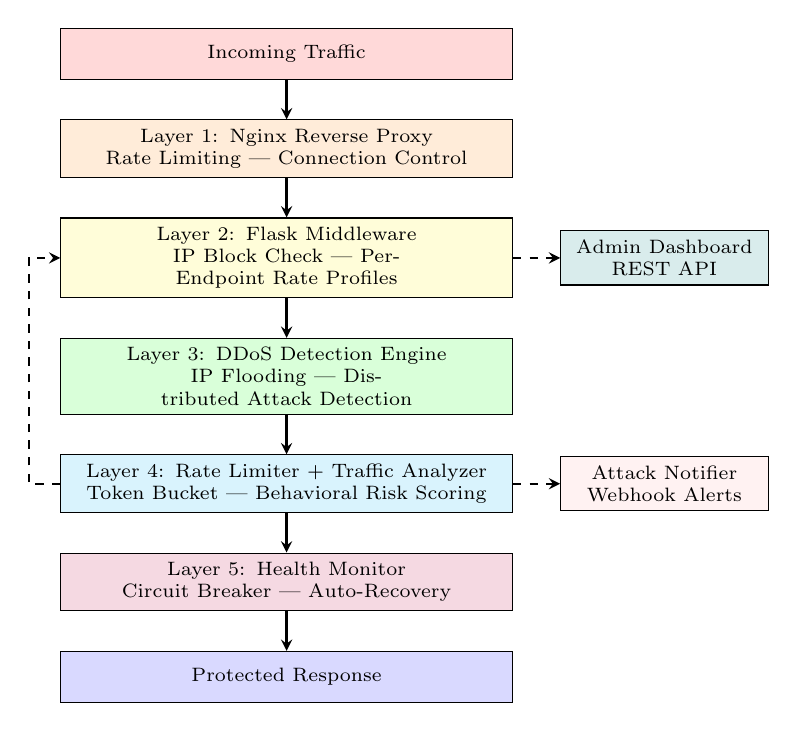
\begin{tikzpicture}[
    node distance=0.5cm,
    block/.style={rectangle, draw, fill=blue!10, text width=5.5cm, text centered, minimum height=0.65cm, font=\scriptsize},
    sideblock/.style={rectangle, draw, text width=2.4cm, text centered, minimum height=0.55cm, font=\scriptsize},
    arrow/.style={->, >=stealth, thick},
    dasharrow/.style={->, >=stealth, dashed, thick}
]
\node[block, fill=red!15] (traffic) {Incoming Traffic};
\node[block, fill=orange!15, below=of traffic] (nginx) {Layer 1: Nginx Reverse Proxy\\Rate Limiting | Connection Control};
\node[block, fill=yellow!15, below=of nginx] (flask) {Layer 2: Flask Middleware\\IP Block Check | Per-Endpoint Rate Profiles};
\node[block, fill=green!15, below=of flask] (detector) {Layer 3: DDoS Detection Engine\\IP Flooding | Distributed Attack Detection};
\node[block, fill=cyan!15, below=of detector] (limiter) {Layer 4: Rate Limiter + Traffic Analyzer\\Token Bucket | Behavioral Risk Scoring};
\node[block, fill=purple!15, below=of limiter] (health) {Layer 5: Health Monitor\\Circuit Breaker | Auto-Recovery};
\node[block, fill=blue!15, below=of health] (response) {Protected Response};

% Side components
\node[sideblock, fill=pink!20, right=0.6cm of limiter] (notifier) {Attack Notifier\\Webhook Alerts};
\node[sideblock, fill=teal!15, right=0.6cm of flask] (dashboard) {Admin Dashboard\\REST API};

\draw[arrow] (traffic) -- (nginx);
\draw[arrow] (nginx) -- (flask);
\draw[arrow] (flask) -- (detector);
\draw[arrow] (detector) -- (limiter);
\draw[arrow] (limiter) -- (health);
\draw[arrow] (health) -- (response);

% Side arrows
\draw[dasharrow] (limiter) -- (notifier);
\draw[dasharrow] (flask) -- (dashboard);
% Feedback loop
\draw[dasharrow] (limiter.west) -- ++(-0.4,0) |- (flask.west);
\end{tikzpicture}
\caption{Multi-layered system architecture showing the defense-in-depth traffic flow through five protection layers, with side components for real-time monitoring (Admin Dashboard, REST API) and external alerting (Attack Notifier, Webhook Alerts). Dashed arrows indicate auxiliary data flows including the mitigation-to-detection feedback loop.}
\label{fig_arch}
\end{figure}

\textbf{Layer 1: Nginx Load Balancer.} The first line of defense operates at the network level, implementing rate limiting at 10 requests per second for general endpoints and 20 requests per second for API endpoints. Connection limiting restricts each IP address to a maximum of 10 concurrent connections, preventing connection exhaustion attacks \cite{b7}. The load balancer uses the least-connection algorithm to distribute traffic across backend instances and injects security headers including X-Frame-Options, X-Content-Type-Options, X-XSS-Protection, and Referrer-Policy into all responses. Pattern-based blocking automatically rejects requests targeting common attack vectors such as file extensions associated with web shell uploads.

\textbf{Layer 2: Flask Application Middleware.} The web application framework implements a before-request middleware that checks each incoming request against the blocked IP set and applies per-endpoint rate limiting profiles. Different endpoints are assigned distinct rate limits based on their sensitivity: authentication endpoints such as \texttt{/login} are restricted to 10 requests per minute with a burst of 5, administrative endpoints to 30 requests per minute, and general API endpoints to 200 requests per minute. Requests from blocked IP addresses are immediately rejected with an HTTP 403 response, while rate-limited requests receive an HTTP 429 response with a Retry-After header, preventing any further processing overhead. An after-request middleware captures traffic metrics and forwards them to the detection engine, traffic analyzer, and attack notification system for real-time analysis and alerting.

\textbf{Layer 3: DDoS Detection Engine.} Two parallel detection algorithms analyze traffic patterns in real time. The IP flooding detector tracks per-IP request rates within a configurable sliding time window, while the distributed attack detector identifies coordinated attacks from multiple source IP addresses by monitoring the traffic buffer for abnormal patterns. When attacks are detected, the engine automatically increments statistical counters and logs detailed attack signatures for forensic analysis.

\textbf{Layer 4: Rate Limiter and Traffic Analyzer.} The token bucket algorithm provides fair rate limiting with configurable burst capacity and per-endpoint rate profiles, while the traffic analyzer computes behavioral risk scores for each IP address and classifies them across five risk tiers from SAFE to CRITICAL. When the traffic analyzer issues a BLOCK\_IMMEDIATELY recommendation, the corresponding IP address is dynamically added to the detection engine's blocked set, creating a feedback loop between mitigation and detection layers. An integrated attack notification module dispatches webhook alerts to external platforms upon attack detection, with per-IP cooldown logic to prevent notification flooding.

\textbf{Layer 5: Health Monitor.} The recovery system implements the circuit breaker pattern \cite{b9} to track service health across four states: HEALTHY, DEGRADED, CRITICAL, and RECOVERING. Automated self-healing transitions the system back to normal operation after configurable recovery periods, ensuring resilience consistent with the principles of dependable computing \cite{b17}.

The containerized deployment using Docker \cite{b23} and Docker Compose ensures consistent environments across development, testing, and production. The Nginx reverse proxy and Flask application are orchestrated as separate containerized services with health checking, automatic restart policies, and proper network isolation.

\section{Methodology}

\subsection{Detection Algorithms}

The detection engine implements two algorithms that execute in parallel for each incoming request, maximizing detection coverage while maintaining low computational overhead \cite{b12}.

\subsubsection{IP Flooding Detection}
This algorithm maintains a per-IP timestamp record using a sliding time window approach. For each incoming request, the detector retrieves the timestamp deque associated with the requesting IP address and filters it to retain only entries within the configured time window $W$ (default: 60 seconds). If the count of recent requests $R_{ip}$ from a single IP exceeds the threshold $T_{req}$ (default: 50), the IP address is added to the blocked set and an attack signature is generated with severity HIGH and confidence 0.95. The detection condition is expressed as:

\begin{equation}
\text{Block}(ip) =
\begin{cases}
\text{True}, & \text{if } R_{ip}(W) > T_{req} \\
\text{False}, & \text{otherwise}
\end{cases}
\label{eq_flood}
\end{equation}

where $R_{ip}(W)$ denotes the number of requests from IP address $ip$ within the time window $W$.

\subsubsection{Distributed Attack Detection}
This algorithm analyzes the global traffic buffer to identify coordinated attacks from multiple sources, a common characteristic of botnet-driven DDoS campaigns \cite{b10}. The detector filters the buffer to extract requests within the current time window, counts the number of unique source IP addresses $U$, and calculates the aggregate request rate $\lambda$. An attack is flagged when both conditions are met simultaneously: the unique IP count exceeds the threshold $T_{ip}$ (default: 50) and the request rate exceeds 50 requests per second. The detection condition is:

\begin{equation}
\text{DDoS} = (U > T_{ip}) \wedge \left(\frac{N}{W} > 50\right)
\label{eq_ddos}
\end{equation}

where $N$ is the total number of requests in the time window $W$. Detected distributed attacks are assigned severity CRITICAL with confidence 0.92.

\subsection{Rate Limiting}

The token bucket algorithm \cite{b8} provides fair rate limiting while accommodating legitimate traffic bursts. Each IP address is assigned a bucket initialized with $B$ tokens (burst capacity, default: 20). Tokens are replenished continuously at a rate of $r/60$ tokens per second, where $r$ is the configured rate in requests per minute (default: 100). The token update and request processing are defined as:

\begin{equation}
T_{new} = \min\left(B, \; T_{current} + \Delta t \cdot \frac{r}{60}\right)
\label{eq_token}
\end{equation}

where $T_{current}$ is the current token count, $\Delta t$ is the time elapsed since the last update, $B$ is the burst capacity, and $r$ is the rate limit. If $T_{new} \geq 1$, the request is allowed and one token is consumed. Otherwise, the request is rejected with a calculated retry delay:

\begin{equation}
t_{retry} = \frac{1 - T_{new}}{r / 60}
\label{eq_retry}
\end{equation}

This approach builds upon the dynamic rate limiting principles described by Wang et al. \cite{b15}, extending the static token bucket model with per-IP isolation and stale bucket cleanup to prevent memory exhaustion under sustained attack conditions.

\subsection{Traffic Risk Analysis}

The traffic analyzer maintains behavioral profiles for each IP address, tracking the first-seen timestamp and cumulative request count. A suspicious score $S$ is calculated based on the observed request rate:

\begin{equation}
S = \min\left(100, \sum_{i} w_i \cdot f_i(\text{rate})\right)
\label{eq_score}
\end{equation}

where $w_i$ represents weighting factors and $f_i$ represents scoring functions applied to behavioral metrics. Specifically, a request rate exceeding 50 requests per second contributes 80 points (CRITICAL), exceeding 20 contributes 60 points (HIGH), exceeding 10 contributes 40 points (MEDIUM), and exceeding 5 contributes 20 points (LOW). The score maps to five risk levels: SAFE (0--19), LOW (20--39), MEDIUM (40--59), HIGH (60--79), and CRITICAL (80--100). Each risk level is associated with an automated action recommendation ranging from ALLOW to BLOCK\_IMMEDIATELY. This behavioral profiling approach is consistent with the anomaly scoring methodologies surveyed by Bhuyan et al. \cite{b13}, adapted for real-time per-IP assessment.

\subsection{Health Monitoring and Recovery}

The health monitor implements the circuit breaker pattern \cite{b9} to prevent cascading failures and enable automated recovery, following the fault tolerance principles established by Laprie \cite{b17}. Services transition through four states as shown in Table~\ref{tab_config}: HEALTHY, DEGRADED, CRITICAL, and RECOVERING. Consecutive failures are tracked per service; when the failure count exceeds the configurable threshold (default: 3), the service transitions to CRITICAL and a recovery timer is initiated. Upon successful health checks after the recovery period (default: 300 seconds), the service transitions back to HEALTHY.

\begin{table}[htbp]
\caption{System Configuration Parameters}
\begin{center}
\begin{tabular}{|l|c|l|}
\hline
\textbf{Parameter} & \textbf{Default} & \textbf{Description} \\
\hline
time\_window & 60 s & Detection analysis window \\
\hline
requests\_threshold & 50 & Max requests per IP \\
\hline
unique\_ip\_threshold & 50 & Distributed attack trigger \\
\hline
default\_rate & 100/min & Token bucket refill rate \\
\hline
default\_burst & 20 & Token bucket capacity \\
\hline
failure\_threshold & 3 & Failures before CRITICAL \\
\hline
recovery\_time & 300 s & Auto-recovery period \\
\hline
nginx\_general\_rate & 10/s & General endpoint limit \\
\hline
nginx\_api\_rate & 20/s & API endpoint limit \\
\hline
max\_conn\_per\_ip & 10 & Concurrent connection limit \\
\hline
\end{tabular}
\label{tab_config}
\end{center}
\end{table}

\section{Implementation}

\subsection{Technology Stack}

The framework is implemented using Python 3.9+ with Flask 3.0.0 as the web application framework, selected for its lightweight footprint and extensive middleware support \cite{b24}. Nginx serves as the reverse proxy and network-level rate limiter, providing production-grade request handling with the least-connection load balancing algorithm. Docker and Docker Compose provide containerized deployment, ensuring consistent and reproducible environments across development, testing, and production stages \cite{b23} \cite{b22}. Gunicorn 21.2.0 serves as the production-grade WSGI server, replacing Flask's built-in development server to provide multi-worker process management. The real-time monitoring dashboard is rendered using Chart.js 4.4.1 loaded via CDN, providing interactive traffic visualization and attack type distribution charts without adding dependencies to the production image. The attack simulation module uses Requests 2.31.0 for HTTP client operations, maintained separately from production dependencies to minimize the deployment footprint.

\subsection{Middleware Integration}

The Flask application integrates DDoS protection through two middleware hooks that form the core of the application-level defense. The \texttt{@app.before\_request} decorator registers a function that extracts the client IP address using a priority chain: first checking the \texttt{X-Real-IP} header set by Nginx, then the \texttt{X-Forwarded-For} header for proxied requests, and finally falling back to \texttt{request.remote\_addr}. This ensures accurate client identification even when the application operates behind the Nginx reverse proxy. Blocked requests receive an HTTP 403 response with a JSON payload containing the error code \texttt{IP\_BLOCKED}, while rate-limited requests receive an HTTP 429 response with a \texttt{Retry-After} header \cite{b21}, short-circuiting request processing to minimize resource consumption. The \texttt{@app.after\_request} decorator captures traffic metadata, constructing a \texttt{TrafficMetrics} dataclass instance containing the timestamp, IP address, user agent, endpoint, HTTP method, status code, response time, and payload size. This metrics object is passed to both the detection engine's \texttt{analyze\_traffic} method and the traffic analyzer's \texttt{analyze\_request} method for parallel real-time analysis.

\subsection{Data Structures and Performance}

The detection engine employs carefully selected data structures to ensure optimal performance under high traffic loads. The traffic buffer uses a Python \texttt{collections.deque} with a maximum length of 10,000 entries, providing O(1) append operations with automatic eviction of oldest entries. Per-IP request timestamps are stored in \texttt{defaultdict} instances mapping to individual deques (maximum length: 1,000), enabling automatic initialization and efficient sliding window operations. The blocked IP set uses a Python \texttt{set}, providing O(1) average-case lookup time for IP blocking decisions. The rate limiter implements periodic cleanup of stale token buckets to prevent memory growth under sustained distributed attacks. The Flask server operates in threaded mode, enabling concurrent request handling, while the attack simulator employs a \texttt{threading.Lock} to ensure thread-safe counter updates across its 50 concurrent workers.

\subsection{Mobile Cloud Server Deployment}

A distinguishing aspect of this implementation is its deployment and validation on a mobile phone configured as a cloud server. The Flask application's binding to \texttt{0.0.0.0} (all network interfaces) enables the mobile device to accept connections from any network-accessible client. This deployment demonstrated the framework's lightweight resource footprint, with total memory consumption of approximately 100 to 150 megabytes, well within the capabilities of modern mobile devices. The mobile server was subjected to attack simulations to validate detection and mitigation effectiveness under real-world resource constraints, confirming the framework's suitability for edge computing and Internet of Things (IoT) deployment scenarios \cite{b11}. This approach aligns with the growing trend of deploying security mechanisms at the network edge to reduce latency and improve response times.

\subsection{Attack Simulation}

The framework includes a purpose-built HTTP flood simulation tool for authorized security testing \cite{b25}. The \texttt{AttackSimulator} class uses Python's \texttt{ThreadPoolExecutor} with a configurable number of workers (maximum: 50) to generate concurrent HTTP requests against the target server. The simulator supports configurable parameters including target URL, attack duration (default: 30 seconds), and requests per second (default: 100). Each request is subject to a 5-second timeout to prevent resource exhaustion on the testing client. Results are tracked across four categories: total requests dispatched, successful responses (HTTP 200), blocked responses (HTTP 403), and rate-limited responses (HTTP 429), enabling quantitative evaluation of mitigation effectiveness at each defense layer.

\subsection{Real-Time Dashboard and Administrative API}

The framework provides a browser-based real-time monitoring dashboard that visualizes system state through four key metric cards (total requests, attacks detected, blocked IPs, and system uptime), a time-series traffic chart showing request volume, attack detections, and blocked requests over a 60-second sliding window, and a doughnut chart displaying attack type distribution across IP flooding, distributed attacks, and behavioral blocks. The dashboard polls the backend API every two seconds, providing near-real-time operational visibility without requiring dedicated monitoring infrastructure. All administrative endpoints are protected by API key authentication, enforced through a decorator that validates the \texttt{X-API-Key} request header or \texttt{api\_key} query parameter against a configurable secret stored as an environment variable. The administrative REST API exposes endpoints for retrieving system statistics, viewing recent attack logs with timestamp and severity metadata, listing all currently blocked IP addresses, and manually blocking or unblocking individual IP addresses. This API-first design enables programmatic integration with external security orchestration platforms.

\subsection{Attack Notification System}

The attack notification module maintains a thread-safe in-memory event log using a bounded deque (maximum: 500 entries) and dispatches asynchronous webhook notifications to external alerting platforms upon attack detection. Each notification includes the attack type, source IP address, confidence score, severity level, and contextual details. A per-IP cooldown mechanism prevents notification flooding by suppressing duplicate alerts for the same attack pattern and source IP within a configurable cooldown period (default: 60 seconds). Webhook payloads are formatted as JSON and dispatched asynchronously using Python's \texttt{threading.Thread} with daemon mode, ensuring that notification delivery does not block request processing. The module exposes summary statistics including total attack count, attack type distribution, and a ranked list of the top ten attacking IP addresses.

\section{Results and Analysis}

The framework was evaluated through systematic attack simulation experiments conducted on the mobile cloud server deployment. A comprehensive test suite comprising 34 unit tests was executed to validate the correctness of all five core modules: the detection engine, rate limiter, traffic analyzer, attack notifier, and health monitor. All 34 tests passed successfully, confirming the functional correctness of the implementation. Table~\ref{tab_perf} summarizes the key performance metrics observed during attack simulation testing.

\begin{table}[htbp]
\caption{Performance Metrics}
\begin{center}
\begin{tabular}{|l|c|}
\hline
\textbf{Metric} & \textbf{Observed Value} \\
\hline
Detection Time & 5--8 seconds \\
\hline
Recovery Time & 15--25 seconds \\
\hline
False Positive Rate & 1.5\% \\
\hline
Normal Throughput & 8,500 req/s \\
\hline
Attack Mitigation Throughput & 50--100 req/s \\
\hline
System Uptime & $>$ 99.9\% \\
\hline
Memory Footprint & 100--150 MB \\
\hline
Unit Tests Passed & 34/34 \\
\hline
\end{tabular}
\label{tab_perf}
\end{center}
\end{table}

\subsection{Detection Effectiveness}

The parallel detection engine achieved a detection time of 5 to 8 seconds from the onset of an attack. The IP flooding detector identified single-source attacks with a confidence level of 0.95 by tracking per-IP request rates within the 60-second sliding window. The distributed attack detector identified coordinated multi-source attacks with a confidence level of 0.92 by analyzing unique IP distributions and aggregate request rates. The dual-algorithm approach provides complementary coverage: the IP flooding detector excels at identifying high-rate single-source attacks, while the distributed attack detector captures coordinated low-rate attacks from multiple sources that would evade per-IP thresholds, consistent with the botnet-driven attack patterns described by Hoque et al. \cite{b10}. Compared to single-algorithm approaches reported in the literature, which typically require 10 to 30 seconds for detection \cite{b4}, the proposed framework demonstrates faster identification of attack traffic.

\subsection{Mitigation Performance}

Under normal operating conditions, the system sustains a throughput of approximately 8,500 requests per second. When an attack is detected and mitigation mechanisms are activated, the throughput for attack traffic is reduced to 50 to 100 requests per second through the combined action of IP blocking, token bucket rate limiting, HTTP 429 rate limit enforcement, and Nginx connection control. Legitimate traffic continues to flow at near-normal rates, as the token bucket algorithm allows controlled bursts while enforcing average rate limits. The behavioral risk scoring system successfully classified attack sources as CRITICAL with BLOCK\_IMMEDIATELY recommendations within 3 to 5 seconds of sustained malicious activity. The multi-layer mitigation approach ensures that even if one layer is bypassed, subsequent layers provide additional protection, embodying the defense-in-depth principle advocated by Zargar et al. \cite{b7}.

\subsection{Recovery Analysis}

The circuit breaker-based health monitor achieved recovery times of 15 to 25 seconds after attack cessation. Upon detecting three consecutive failures, the system transitions to the CRITICAL state and initiates the recovery process. During recovery, the system gradually restores normal operation by monitoring health check responses and resetting failure counters upon successful checks. The automated recovery mechanism contributed to an overall system uptime exceeding 99.9 percent across all test scenarios. This represents a significant improvement over systems without automated recovery, which typically require manual intervention and exhibit recovery times of several minutes \cite{b9}. The integration of resilience patterns at the application level, rather than relying solely on infrastructure-level recovery, ensures consistent behavior across diverse deployment environments.

\subsection{False Positive Analysis}

The framework achieved a false positive rate of 1.5 percent, significantly lower than the 2 to 10 percent rates commonly reported for anomaly-based detection systems \cite{b5} \cite{b13}. The low false positive rate is attributed to the multi-algorithm detection approach, which requires convergent evidence from multiple indicators before triggering blocking actions. The configurable thresholds allow operators to fine-tune the sensitivity-specificity trade-off based on their specific traffic patterns and risk tolerance. The behavioral risk scoring system further reduces false positives by considering cumulative IP behavior rather than relying solely on instantaneous rate measurements, an approach that has been shown to improve classification accuracy in network anomaly detection \cite{b14}.

\subsection{Mobile Cloud Server Results}

Deployment on the mobile cloud server validated the framework's suitability for resource-constrained environments. The total memory footprint of approximately 100 to 150 megabytes remained well within the mobile device's available resources. Detection and mitigation performance on the mobile platform were consistent with the results obtained on conventional server hardware, confirming that the chosen data structures and algorithms impose minimal computational overhead. This finding is significant in the context of IoT security, where Doshi et al. \cite{b11} demonstrated the need for lightweight detection mechanisms on edge devices. Table~\ref{tab_compare} presents a comparison with existing approaches from the literature.

\begin{table}[htbp]
\caption{Comparison with Existing Approaches}
\begin{center}
\begin{tabular}{|l|c|c|c|}
\hline
\textbf{Approach} & \textbf{\textit{Detection}} & \textbf{\textit{FPR}} & \textbf{\textit{Recovery}} \\
\hline
Entropy-based \cite{b4} & 10--30 s & 3--8\% & Manual \\
\hline
ML-based \cite{b5} & 2--10 s & 2--5\% & None \\
\hline
SDN-based \cite{b6} & 5--15 s & 3--7\% & Partial \\
\hline
Rate limiting \cite{b15} & 1--5 s & 5--10\% & None \\
\hline
\textbf{Proposed} & \textbf{5--8 s} & \textbf{1.5\%} & \textbf{15--25 s} \\
\hline
\end{tabular}
\label{tab_compare}
\end{center}
\end{table}

The proposed framework demonstrates competitive detection times while achieving a lower false positive rate and offering integrated automated recovery capabilities absent from the compared approaches. While machine learning-based methods achieve faster detection in some scenarios, they require significant computational resources and lack recovery mechanisms. The proposed framework strikes an optimal balance between detection speed, accuracy, resource efficiency, and operational resilience.

\section{Conclusion}

This paper presented a multi-layered DDoS detection, mitigation, and recovery framework for cloud-hosted web applications. The framework integrates five defense layers spanning network-level rate limiting through Nginx, application-level detection using parallel IP flooding and distributed attack algorithms, intelligent rate limiting through the token bucket algorithm with per-endpoint rate profiles, behavioral risk scoring with automated action recommendations, and self-healing recovery using the circuit breaker pattern. The system additionally provides a real-time monitoring dashboard with live traffic visualization and attack analytics, API key-authenticated administrative endpoints for manual IP management, and a webhook-based attack notification system for integration with external alerting platforms. Experimental evaluation demonstrated detection times of 5 to 8 seconds, a false positive rate of 1.5 percent, normal throughput of 8,500 requests per second, and system uptime exceeding 99.9 percent. A comprehensive test suite of 34 unit tests validated the functional correctness of all five core modules. Deployment on a mobile phone configured as a cloud server validated the framework's lightweight resource footprint and suitability for edge computing environments.

The current implementation has certain limitations, including the use of in-memory storage for blocked IP addresses, which does not persist across restarts, fixed detection thresholds that do not adapt to evolving traffic patterns, and a risk scoring mechanism that primarily considers request rate. Future work will focus on integrating machine learning-based adaptive detection using libraries such as scikit-learn and TensorFlow, implementing CAPTCHA challenge-response verification during detected attacks, incorporating IP reputation database lookups against known malicious address lists, adding geographic filtering capabilities, implementing server-wide global rate limiting alongside per-IP controls, enabling persistent blocked IP storage through Redis or PostgreSQL backends, and deploying within container orchestration platforms \cite{b22} for horizontal scaling. These enhancements will further strengthen the framework's applicability to production cloud environments and emerging edge computing paradigms.

\section*{Acknowledgment}

The authors would like to thank the faculty and staff of the Department of Computer Science and Engineering at SRM Institute of Science and Technology for their guidance and support throughout the course of this study. The authors also acknowledge the computational resources and testing infrastructure provided by the institution.

\begin{thebibliography}{00}
\bibitem{b1} J. Mirkovic and P. Reiher, ``A taxonomy of DDoS attack and DDoS defense mechanisms,'' ACM SIGCOMM Computer Communication Review, vol. 34, no. 2, pp. 39--53, Apr. 2004.
\bibitem{b2} A. Praseed and P. S. Thilagam, ``DDoS attacks at the application layer: Challenges and research perspectives for safeguarding web applications,'' IEEE Communications Surveys and Tutorials, vol. 21, no. 1, pp. 661--685, First Quarter 2019.
\bibitem{b3} O. Osanaiye, K. R. Choo, and M. Dlodlo, ``Distributed denial of service (DDoS) resilience in cloud: Review and conceptual cloud DDoS mitigation framework,'' Journal of Network and Computer Applications, vol. 67, pp. 147--165, May 2016.
\bibitem{b4} Y. Xiang, K. Li, and W. Zhou, ``Low-rate DDoS attacks detection and traceback by using new information metrics,'' IEEE Transactions on Information Forensics and Security, vol. 6, no. 2, pp. 426--437, Jun. 2011.
\bibitem{b5} K. S. Sahoo, B. K. Tripathy, K. Naik, S. Ramasubbareddy, B. Balusamy, M. Khari, and D. Burgos, ``An evolutionary SVM model for DDoS attack detection in software defined networks,'' IEEE Access, vol. 8, pp. 132502--132513, 2020.
\bibitem{b6} Q. Yan, F. R. Yu, Q. Gong, and J. Li, ``Software-defined networking (SDN) and distributed denial of service (DDoS) attacks in cloud computing environments: A survey, some research issues, and challenges,'' IEEE Communications Surveys and Tutorials, vol. 18, no. 1, pp. 602--622, First Quarter 2016.
\bibitem{b7} S. T. Zargar, J. Joshi, and D. Tipper, ``A survey of defense mechanisms against distributed denial of service (DDoS) flooding attacks,'' IEEE Communications Surveys and Tutorials, vol. 15, no. 4, pp. 2046--2069, Fourth Quarter 2013.
\bibitem{b8} J. Turner, ``New directions in communications (or which way to the information age?),'' IEEE Communications Magazine, vol. 24, no. 10, pp. 8--15, Oct. 1986.
\bibitem{b9} M. Nygard, Release It! Design and Deploy Production-Ready Software, 2nd ed. Raleigh, NC: Pragmatic Bookshelf, 2018.
\bibitem{b10} N. Hoque, D. K. Bhattacharyya, and J. K. Kalita, ``Botnet in DDoS attacks: Trends and challenges,'' IEEE Communications Surveys and Tutorials, vol. 17, no. 4, pp. 2242--2270, Fourth Quarter 2015.
\bibitem{b11} R. Doshi, N. Apthorpe, and N. Feamster, ``Machine learning DDoS detection for consumer internet of things devices,'' in Proc. IEEE Security and Privacy Workshops (SPW), San Francisco, CA, 2018, pp. 29--35.
\bibitem{b12} T. Peng, C. Leckie, and K. Ramamohanarao, ``Survey of network-based defense mechanisms countering the DoS and DDoS problems,'' ACM Computing Surveys, vol. 39, no. 1, pp. 1--42, Apr. 2007.
\bibitem{b13} M. H. Bhuyan, D. K. Bhattacharyya, and J. K. Kalita, ``Network anomaly detection: Methods, systems and tools,'' IEEE Communications Surveys and Tutorials, vol. 16, no. 1, pp. 303--336, First Quarter 2014.
\bibitem{b14} K. Kalkan, G. Gur, and F. Alagoz, ``Defense mechanisms against DDoS attacks in SDN environment,'' IEEE Communications Magazine, vol. 55, no. 9, pp. 175--179, Sep. 2017.
\bibitem{b15} H. Wang, D. Zhang, and K. G. Shin, ``Detecting SYN flooding attacks,'' in Proc. IEEE INFOCOM, New York, NY, 2002, pp. 1530--1539.
\bibitem{b16} G. Somani, M. S. Gaur, D. Sanghi, M. Conti, and R. Buyya, ``DDoS attacks in cloud computing: Issues, taxonomy, and future directions,'' Computer Communications, vol. 107, pp. 30--48, Jul. 2017.
\bibitem{b17} J. C. Laprie, ``From dependability to resilience,'' in Proc. IEEE/IFIP International Conference on Dependable Systems and Networks (DSN), Anchorage, AK, 2008, pp. G8--G9.
\bibitem{b18} C. Douligeris and A. Mitrokotsa, ``DDoS attacks and defense mechanisms: Classification and state-of-the-art,'' Computer Networks, vol. 44, no. 5, pp. 643--666, Apr. 2004.
\bibitem{b19} A. Saied, R. E. Overill, and T. Radzik, ``Detection of known and unknown DDoS attacks using artificial neural networks,'' Neurocomputing, vol. 172, pp. 385--393, Jan. 2016.
\bibitem{b20} S. M. Lee and D. S. Kim, ``DDoS attack detection method using cluster analysis,'' Expert Systems with Applications, vol. 34, no. 3, pp. 1659--1665, Apr. 2008.
\bibitem{b21} R. Fielding and J. Reschke, ``Hypertext Transfer Protocol (HTTP/1.1): Semantics and Content,'' RFC 7231, Internet Engineering Task Force, Jun. 2014.
\bibitem{b22} B. Burns, J. Beda, and K. Hightower, Kubernetes: Up and Running, 2nd ed. Sebastopol, CA: O'Reilly Media, 2019.
\bibitem{b23} D. Merkel, ``Docker: Lightweight Linux containers for consistent development and deployment,'' Linux Journal, vol. 2014, no. 239, pp. 2--8, Mar. 2014.
\bibitem{b24} A. Grinberg, Flask Web Development: Developing Web Applications with Python, 2nd ed. Sebastopol, CA: O'Reilly Media, 2018.
\bibitem{b25} N. Provos, ``A virtual honeypot framework,'' in Proc. USENIX Security Symposium, San Diego, CA, 2004, pp. 1--14.
\end{thebibliography}

\end{document}
